% zscore question for Jeff
\documentclass[10pt,letterpaper]{article}
\usepackage[top=0.85in,left=2.75in,footskip=0.75in]{geometry}

% Use adjustwidth environment to exceed column width (see example table in text)
\usepackage{changepage}

% Use Unicode characters when possible
\usepackage[utf8]{inputenc}

% textcomp package and marvosym package for additional characters
\usepackage{textcomp,marvosym}

% fixltx2e package for \textsubscript
\usepackage{fixltx2e}

% amsmath and amssymb packages, useful for mathematical formulas and symbols
\usepackage{amsmath,amssymb}

% cite package, to clean up citations in the main text. Do not remove.
\usepackage{cite}

% Use nameref to cite supporting information files (see Supporting Information section for more info)
\usepackage{nameref,hyperref}

% line numbers
\usepackage[right]{lineno}

% ligatures disabled
\usepackage{microtype}
\DisableLigatures[f]{encoding = *, family = * }

% rotating package for sideways tables
\usepackage{rotating}

% Remove comment for double spacing
\usepackage{setspace} 
\doublespacing

% Text layout
\raggedright
\setlength{\parindent}{0.5cm}
\textwidth 5.25in 
\textheight 8.75in

% Bold the 'Figure #' in the caption and separate it from the title/caption with a period
% Captions will be left justified
\usepackage[aboveskip=1pt,labelfont=bf,labelsep=period,justification=raggedright,singlelinecheck=off]{caption}

% Use the PLoS provided BiBTeX style
\bibliographystyle{plos2015}

% Remove brackets from numbering in List of References
\makeatletter
\renewcommand{\@biblabel}[1]{\quad#1.}
\makeatother

% Leave date blank
\date{}

% Header and Footer with logo
\usepackage{lastpage,fancyhdr,graphicx}
\usepackage{epstopdf}
\pagestyle{myheadings}
\pagestyle{fancy}
\fancyhf{}
\lhead{
\includegraphics[width=2.0in]{PLOS-submission.eps}}
\rfoot{\thepage/\pageref{LastPage}}
\renewcommand{\footrule}{\hrule height 2pt \vspace{2mm}}
\fancyheadoffset[L]{2.25in}
\fancyfootoffset[L]{2.25in}
\lfoot{\sf PLOS}

%% Include all macros below

\newcommand{\lorem}{{\bf LOREM}}
\newcommand{\ipsum}{{\bf IPSUM}}

%% END MACROS SECTION


%%% Begin BWP
%\usepackage{amsmath, amsthm, amssymb, wasysym, graphicx}
%\usepackage[small, hang, bf]{caption}
%\usepackage{natbib}
%\renewcommand\cite{\citep}
%\newcommand\citepossessive[1]{\citeauthor{#1}'s \citeyearpar{#1}}
\newcommand\eq[1]{Eq.~\ref{#1}}
\newcommand\fig[1]{Fig.~\ref{#1}}
\newcommand\sref[1]{Section~\ref{#1}}
\let\oldmarginpar\marginpar
\renewcommand{\marginpar}[1]{\oldmarginpar{\linespread{1}\scriptsize{#1}}}

% PLOS wants \paragraph for some reason...
\renewcommand{\subsubsection}[1]{\paragraph{#1}}

\setlength{\marginparwidth}{55mm}


\newcommand\argmin{\mathop{\textrm{{\rm argmin}}}\limits}
\newcommand{\noprint}[1]{}


\hyphenation{cross-valid-ation}
%%% End BWP


\begin{document}
\vspace*{0.35in}

% Title must be 250 characters or less.
% Please capitalize all terms in the title except conjunctions, prepositions, and articles.
\begin{flushleft}
{\Large
\textbf\newline{A Fast and Accurate Zebra Finch Syllable Detector}
}
\newline
% Insert author names, affiliations and corresponding author email (do not include titles, positions, or degrees).
\\
Ben Pearre\textsuperscript{1,a,\textcurrency},
L.~Nathan Perkins\textsuperscript{1,b},
Jeffrey E.~Markowitz\textsuperscript{1,c},
Timothy J.~Gardner\textsuperscript{1,d}
\\
\bigskip
\textsuperscript{1} Department of Biology, Boston University, Boston, Massachusetts, United States of America
\\
\bigskip

% Insert additional author notes using the symbols described below. Insert symbol callouts after author names as necessary.
% 
% Remove or comment out the author notes below if they aren't used.
%
% Primary Equal Contribution Note
%\Yinyang These authors contributed equally to this work.
Author \textsuperscript{a}~contributed the original Matlab and LabView implementations and most of the manuscript.
\textsuperscript{b}~contributed the Swift implementation and its description herein, helped debug the training code, and measured the timing for most of the detectors.
\textsuperscript{c}~wrote several types of filterbank software against which we compared, made suggestions for the neural network detector, and prepared the final version of the Matlab code for distribution.
\textsuperscript{d}~provided a stream of suggested techniques, metrics, and goals.

% Additional Equal Contribution Note
% Also use this double-dagger symbol for special authorship notes, such as senior authorship.
%\ddag These authors also contributed equally to this work.

% Current address notes
%\textcurrency a Insert current address of first author with an address update
% \textcurrency b Insert current address of second author with an address update
% \textcurrency c Insert current address of third author with an address update

% Deceased author note
%\dag Deceased

% Group/Consortium Author Note
%\textpilcrow Membership list can be found in the Acknowledgments section.

% Use the asterisk to denote corresponding authorship and provide email address in note below.
\textsuperscript{\textcurrency} Corresponding author: bwpearre@gmail.com (BP)

\end{flushleft}

\reversemarginpar
%%% End PLOS header template



\begin{abstract}
  The song of the adult male zebra finch is strikingly stereotyped.  Efforts to
  understand motor output, pattern generation, and learning have taken
  advantage of this consistency by investigating the bird's ability to
  modify specific parts of song under external cues, and by examining
  timing relationships between neural activity and vocal output.  Such
  experiments require that precise moments during song be identified in real time
  as the bird sings.  Various syllable-detection methods exist, but
  many require special hardware, software, and know-how, and details
  on their implementation and performance are scarce.  We present an
  accurate, versatile, and fast syllable detector that can control
  hardware at precisely timed moments during zebra finch song.  Many
  moments during song can be isolated and detected with false negative and
  false positive rates well under 0.5\% and 0.01\% respectively. The
  detector can run on a stock Mac Mini with triggering delay of less than a millisecond and a jitter of $\sigma\approx 2$
  milliseconds.
\end{abstract}

\linenumbers

\section{Introduction}

The adult zebra finch ({\em Taeniopygia guttata}) sings a song made up
of 2--6 syllables, with longer songs taking on the order of a
second. The song may be repeated hundreds of times per day, is
almost identical each time, and several brain areas reflect this consistency in highly stereotyped neural firing patterns. This consistency makes the zebra finch one of the most popular models for the study of the neural basis of learning, audition, and
control.

This consistency allows a variety of experiments if precise moments
in song can reliably be detected quickly enough to trigger other
apparatus during singing.  A common area of study with this song-triggering technique is the anterior forebrain pathway (AFP), a homologue of mammalian basal ganglia consisting of a few distinct brain areas concerned with the acquisition and learning of song.  For example, \cite{Kao2005} stimulated the
lateral magnocellular nucleus of the anterior nidopallium (LMAN)---the
output nucleus of the AFP---at precisely
timed moments during song and showed that this area repeatably
controls specific variables in song output.  \cite{Andalman2009} played a disruptive sound during renditions of a syllable that were slightly above (or below) its
average pitch, and showed
that AFP produces a corrective signal to bias song away from those disruptions.  \cite{Warren2011} showed
that that AFP transfers this signal to the robust nucleus of the arcopallium (RA) using NMDA-receptor--mediated glutamatergic
transmission. By looking at song recovery after applying the same
pitch-shift paradigm, \cite{Canopoli2014} showed that the caudal
medial nidopallium is implicated in memorising or recalling a recent
song target, but for neither auditory processing nor directed motor
learning.

% THEIR WORDS: (NCM, a high auditory area) impaired recovery of the original pitch even several weeks after withdrawal of the reinforcing stimuli. Because NCM lesions spared both successful noise-avoidance behavior and birds' auditory discrimination ability, our results show that NCM is not needed for directed motor changes or for auditory discriminative processing, but is implied in memorizing or recalling the memory of the recent song target.


Despite the power and versatility of such experiments, there is no standard syllable detector.  Considerations include:
\begin{description}
\item[Accuracy:] How often does the system produce false positives or false negatives?
\item[Latency:] The average delay between the target syllable being sung and the detection.
\item[Jitter:] The amount that latency changes from instance to instance of song.  Our measure of jitter is the standard deviation $\sigma$ of latency.
\item[Versatility:] Is detection possible at ``difficult'' syllables?
\item[Ease of use:] How automated is the process of programming a detector?
\item[Cost:] What are the hardware and software requirements?
\end{description}

A variety of syllable-triggering systems have been used, but few have been documented or characterised in detail.  In 1999, \cite{Leonardo1999}  used groups of IIR filters with hand-tuned logical operators.  Their system had a latency of 50 or 100 milliseconds (ms), and they do not report on jitter or accuracy.  As access to computational resources has improved, approaches have changed: in 2009, \cite{Andalman2009} still used hand-tuned filters, but ran them on a Tucker-Davis Technologies digital signal processor.  They report a latency of around 4 ms, but as with other filter bank techniques, it is not strictly a syllable detector but rather a pitch and timbre detector---it cannot identify a frequency sweep, or distinguish a short chirp from a long one---and thus requires careful selection of target syllables.  Furthermore, the method is neither inexpensive nor, based on our experience with a similar technique, accurate.  \cite{Keller2009} applied a neural network to a spectral image of song.  They report a latency of 4.3 ms, but further implementation and performance details are not available.  In 2011, \cite{Warren2011} matched spectral templates to stable portions of syllables in 8-ms segments.  They report a jitter of 4.5 ms, and false-negative and false-positive rates of up to 2\% and 4\%, respectively.  Hardware requirements and ease of use were not reported.  In 2013, \cite{Skocik2013} described in detail a system that matches spectral images of template syllables using a correlation coefficient.  With a fast desktop (Intel i7 six-core) running Linux and equipped with a National Instruments data acquisition card, it boasts a hardware-only (not accounting for the time taken to compute a match with a syllable) latency and jitter of just a few microseconds, and the detection computation they use should not much increase that.  Drawbacks are that some hand-tuning is still required, and that they report false-negative rates around 4\% and 7\% for zebra finches and Bengalese finches respectively, measured on a small dataset.  In much other work, an allusion is made to a syllable detector, but no further information is provided.

We developed a standalone detector that learns to match moments in the
song using a neural network applied to the song spectrogram, and
outputs a TTL pulse at the chosen moment. The approach consists of
three steps:

\begin{enumerate}
\item Record and align a corpus of training songs.  The technique has been published in \cite{Poole2012}.
\item Choose one or more instants in the song that should create a trigger event, and train a
  neural network to recognise them. This step is carried out offline.  While any neural network software would produce equivalent results, we used Matlab 2015b's neural network toolbox.
\item Once trained and saved, the neural network is used by a realtime
  detection program that listens to an audio signal and indicates detection of the target
  syllables via a TTL pulse.  We present three implementations that trade off hardware requirements, ease of maintenance, and performance.
\end{enumerate}
This method makes the following contributions:
\begin{itemize}
\item Fast: sub-millisecond latencies, with jitter around 2 ms.
\item Accurate: false positive rates under 0.02\% and false negative rates under 0.5\% for a variety of syllables.  Balancing these rates depends on a single relative-cost parameter.
\item State-of-the-art performance with default parameters.
\item Runs on inexpensive hardware.
\item Described in detail here, with reference implementations provided and benchmarked.
\end{itemize}

%We present the method in Section~\ref{sec:method}.  Section~\ref{sec:results} presents our measurements.
%We
%conclude in Section~\ref{sec:conclusion}, and point to software
%resources in Appendix~\ref{sec:resources}.


\section{Materials and Methods}
\label{sec:method}


\subsection{Learning a detector}

We begin with a few hundred recordings of a given bird's song, in this
case made inside a sound-isolating chamber in which was mounted a
recording microphone (Audio-Technica AT803).  The songs are
time-aligned as described in \cite{Poole2012}.

\begin{figure}
  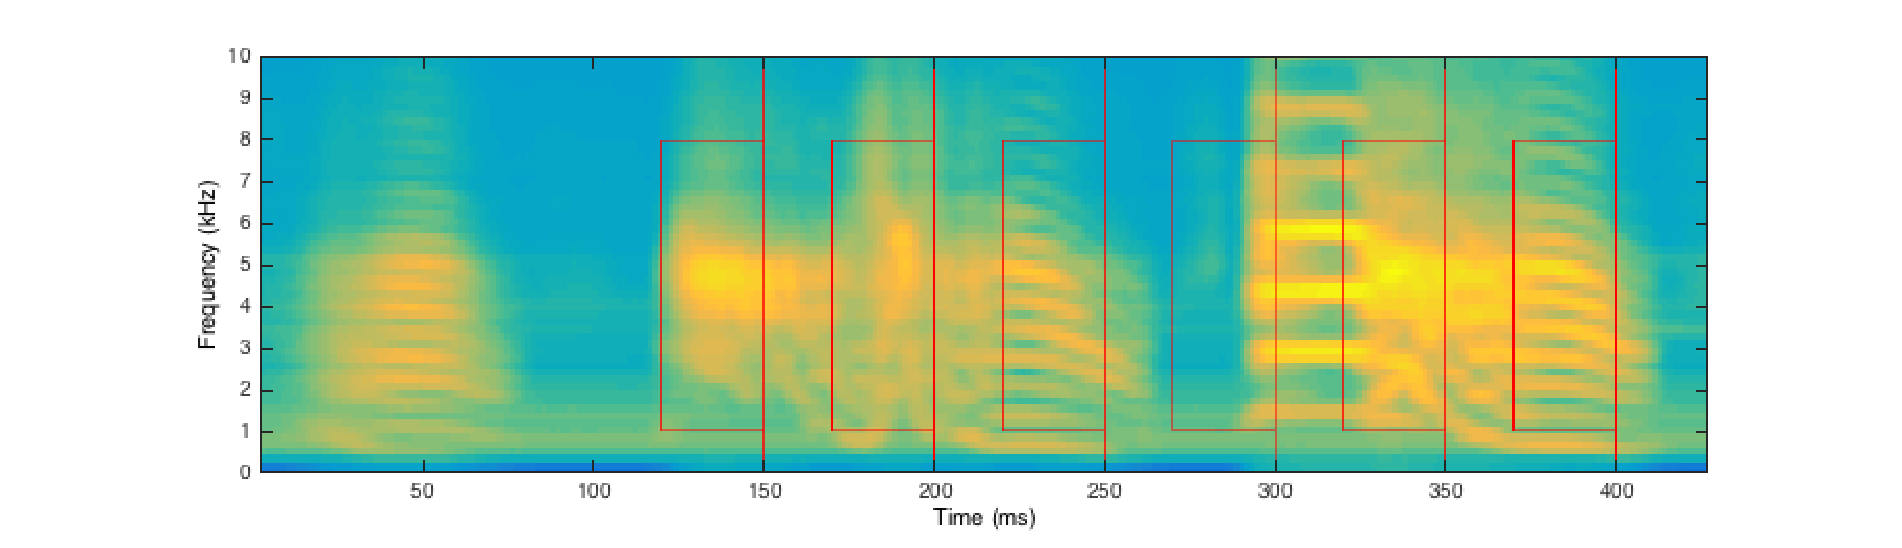
\includegraphics[width=\textwidth]{6syllables}
  \caption{This image was made by superposing the spectra of our 2818 aligned songs.  Our example detection points, $t^*_1\ldots t^*_6$, are shown as red lines, with the recognition regions (30 ms $\times$ 1--8 kHz) marked as rectangles.}
  \label{fig:song}
\end{figure}

We rely on two circular buffers:
\begin{description}
\item[Audio buffer:] This contains the most recent audio samples, and is of the length required to compute the Fast Fourier Transform (FFT)---usually 256 samples.
\item[FFT buffer:] The results of each new FFT are placed here.  It contains the $n_\textrm{fft}$ most recent FFTs, which will serve as inputs to the neural network (described below).
\end{description}

Audio is recorded at some sample rate $1/t_\mathrm{sample}$ (for example, 44.1 kHz), and new data are appended to the circular audio buffer.

The spectrogram is computed at regular intervals---the useful range
seems to be roughly 1--5 milliseconds, which we refer to as the frame
interval $t_\textrm{fft}$.  At each frame, a spectrum is computed from the
most recent 256 audio samples in the audio buffer, and the result is appended to the FFT buffer.  For example, if $t_\textrm{fft}=1$ ms and the recording sample rate $1/t_\textrm{sample}=40$ kHz, then in order to compute a new FFT, $40000\cdot 0.001=40$ new audio samples must be appended to the audio buffer, the FFT is computed using the most recent 256 samples in that buffer, and the result is appended to the FFT buffer.  Over time, the successive spectra will look something
like \fig{fig:song}.

Note that this results in time being discretised into chunks of length
$t_\mathrm{fft}$.  Because each Fourier transform computation contains
a small number $n_\mathrm{fft}$ of new audio samples (in the example
above, 40 new samples and $256-40$ that have already been examined),
we tried implementing the Sliding Discrete Fourier transform (SDFT)
\cite{Jacobsen2003SlidingDFT}.  This allows
$t_\textrm{fft}=t_\textrm{sample}$.  Practically, the operating system
retrieves new audio samples from the hardware several at a time, so
the full benefit of the SDFT is difficult to see in practice.
Furthermore, we found that FFT implementations are sufficiently highly
optimised that discretising time into chunks of $t_\mathrm{fft}$ as we
have done produced similar results with lower software development
effort.

When using consumer audio hardware that operates best at 44.1 kHz, the requested frame interval may not line up with the sample rate, so
the actual frame interval may be different from the indended.  For
example, at 44.1 kHz a 1-ms frame interval requires a new FFT
every 44.1 samples.  This must be rounded to 44 samples, resulting in
$t_\textrm{fft}=\lfloor 44.1 \rceil / 44.1 \approx 0.9977$ ms.

One or more target moments during the song must be chosen.  Our interface
presents the time-aligned spectrogram averaged over training songs,
and requires manual input of the target times, $t^*$.  Then we assemble the
training set from the song data, train the network, compute optimal
output unit thresholds, and save the network object and an audio test
file.

\subsubsection{Recognition region}
\label{sec:recognitionregion}

The neural network's inputs are the FFT values from a rectangular
region of the spectrogram covering a predefined range of frequency values $F$ (for example, 1--8 kHz) at
some number of the most recent frames $n_\textrm{fft}$.  Any time $t$ falls within one of the frames, $\tau(t)$, and $t-t_\textrm{fft}$ falls within the previous frame.  The recognition region that the neural network receives as input consists of the spectrogram values over $F$ at $\tau(t)$ and those from the contiguous set of recent frames: $T = \{$ $\tau(t)$, $\tau(t-t_\textrm{fft})$, $\tau(t-{2t_\textrm{fft}})\ldots$ $\tau(t-n_\textrm{fft}t_\textrm{fft})\}$.  We have found that a 30-ms time window (which will
yield $n_\textrm{fft} = |T|=\lfloor 30\textrm{ ms}/t_\textrm{fft}\rceil$ frames) of frequencies
spanning 1--8 kHz works well for most syllables.

Six examples of chosen target moments in the song, and their corresponding recognition regions $F$ and $T$, are shown in \fig{fig:song}.

%% \subsubsection{Song micro-realignment}

%% As conditions change, and especially during undirected song, syllable
%% length and relative timing may vary slightly, which introduces
%% variations in the precise timing of each syllable. The alignment
%% software we use ensures that songs are aligned at the point midway
%% through the song, but if the target syllable is not at that point, it
%% is helpful to re-align the songs at the point of interest.  This may
%% be accomplished by looking for peaks in the correlation of the
%% time-domain signal with the song whose spectrogram is closest to
%% average over the training set.\marginpar{I hope that's the right thing
%%   to do. Seems to work, anyway\dots}


\subsubsection{Building the training set}

The training set is created in a fashion typical for neural networks:
at each time frame $t$ the rectangular $|F|\times |T|$ recognition
region in the spectrogram as of time $t$ is reshaped into a vector $\xi_t$, which will
have length $|F||T|$ and contain the spectra in $F$ taken at all of the times in the set $T$: from $\tau(t-n_\textrm{fft}t_\textrm{fft})$ to $\tau(t)$.  These vectors are placed into a training
matrix, $\Xi$, such that each column $\xi_t$ holds the contents of the
recognition region---containing multiple columns from the spectrogram---as of one value of $t$

Training targets $y_t$ are vectors with one element for each desired detection syllable.  That element is, roughly, 1 if the input vector comes from the
target time ($t=t^*$), 0 otherwise, for each target syllable (of which there may be any number, although they increase training time, and in our implementations the number of distinct output pulses is constrained by hardware).  Since the song
alignment may not be perfect, due to sample aliasing, and because the song spectrogram appears not to vary faster than the frame rate we chose, a strict binary target may ask the network to learn that, of two practically identical frames, one should be a match and the other not. Thus it is preferable to spread the target
in time, such that at the target moment it is 1,
and at neighbouring moments it is nonzero. We found that a Gaussian
smoothing kernel around the target time with a standard deviation of 2 ms serves well.

\noprint{
  % I screwed up: the results are without cage noise.  Rather than repeat all measurements, let's just not mention it.
  With inputs well outside the space on which a neural network has been
trained, its outputs will be essentially random. In order to reduce
the false positive rate it is useful to provide negative training
examples that include silence, cage noise, non-song vocalisations, and
perhaps songs from other birds.  We have found that training with
as low as a 1:1 ratio of non-song to song yields excellent results,
although this will depend on the makeup of the non-song data.
}

\subsubsection{Normalisation}

In order to present consistent and meaningful inputs to the neural network, we normalise the incoming data stream so that changes in the song structure of the sound are emphasised over changes in volume, and to maximise the effectiveness of the neural network's training algorithm...

The first normalisation step is designed to eliminate differences in amplitude due to changes in the bird's location and other variations in recording.  Each recognition region vector $\xi_t$---during training, each {\em column} of the training matrix $\Xi$---is normalised using Matlab's {\tt zscore} function $\hat{\xi}_t = (\xi_t - \mu_{\xi_t}) / \sigma_{\xi_t}$, so that the content of each window has mean $\mu_{\hat{\xi}_t}=0$ and  standard deviation $\sigma_{\hat{\xi}_t}=1$.

The second step is designed to ensure that the neural network's inputs have a range and distribution for which the training function can easily converge.  Each element $i$ of $\hat{\xi}$ is normalised across the entire training set---each {\em row} of $\Xi$---in the same way: $\check{\xi}^i = (\hat{\xi}^i - \mu_{\hat{\xi}^i})/\sigma_{\hat{\xi}^i}$, so that the values of that point across the whole training set have mean $\mu_{\check{\xi}^i}=0$ and standard deviation $\sigma_{\check{\xi}^i}=1$.  This is accomplished during training by setting Matlab's neural network toolbox normalisation scheme to {\tt mapstd}, and the scaling transform is saved as part of the network object used by the realtime detector so that it may be applied to unseen data at runtime.

These two normalisation steps provide a set of inputs that are more
robust to outliers and less likely to produce false positives during 
silence than other normalisation schemes, such as 
linear or L\textsubscript{2} normalisation.

\subsubsection{Neural Networks}

While any learned classifier might suffice, we chose a two-layer feedforward neural network.  In brief, our network takes an input vector $\xi_t$---as described above---and produces an output vector $y_t$, and when any element of $y_t$ is above a threshold (described below), the detector reports a detection event.  The network uses two matrices of weights, $W_0$ and $W_1$, and two vectors of biases, $b_0$ and $b_1$.  The first takes the input $\xi_t$ to an intermediate stage---the ``hidden layer'' vector.  To each element of this vector is applied a nonlinear squashing function such as {\tt tanh}, and then the second weight matrix $W_1$ is applied.  This produces output $y_t$:
\begin{equation*}
  y_t = W_1 \cdot \tanh (W_0 \cdot \xi_t + b_0) + b_1
\end{equation*}
The elements of each matrix are learned by back-propagation of errors over a training set.  A more detailed explanation of neural networks may be found in \cite{hkp}.

Essentially, after training, the network is available in the form of the two matrices $W_0$ and $W_1$ and the two vectors $b_0$ and $b_1$, and running the network consists of two matrix multiplications, two vector additions and the application of the squashing function.

\subsubsection{Training the network}

The network is trained using Matlab's neural network toolbox. We tried
a variety of feedforward neural network geometries, from simple
1-layer perceptrons to geometries with many hidden
nodes, as well as autoencoders. Perhaps surprisingly, even the former yields excellent results
on many syllables, but a 2-layer perceptron with a very small hidden
layer---with a unit count 2-4 times the number of target
syllables---was a good compromise between accuracy and training
speed. For more variable
songs, deep structure-preserving networks may be more appropriate, but
they are slow to train and unnecessary for zebra finch song.

We used the Levenburg-Marquardt
algorithm, which is the Matlab toolbox's default.  It is a fast algorithm, but is memory-intensive, so
many target syllables or high FFT frame rates require a large
amount of RAM and increase training time to hours. Other training
algorithms that use less RAM are much slower, and by default they will
often terminate prematurely due to their performance gradient
going to 0.

\subsubsection{Computing optimal output thresholds}
\label{sec:optimalthresholds}
After the network is trained, outputs of the network for any input
are now available, and will be in (or, due to noisy inputs and imperfect training, close to) the
interval (0, 1). We must choose a threshold above which the output is
considered a positive detection. Finding the optimal threshold
requires two choices. The first is the relative cost of false
negatives to false positives, $C_n$. The second is the acceptable time
interval: if the true event occurs at time $t$, and the detector
triggers at any time $t\pm\Delta t$, then it is considered a correct
detection. Then the optimal detection threshold $\tau$ is the one that
minimises $\textrm{[false positives]} +C_n\cdot\textrm{[false negatives]}$
over the training set, using the definitions of false positives and
negatives given in Section~\ref{sec:accuracy}. Since large
portions of the cost function are flat, hillclimbing is ineffective.  Random-restart hillclimbing
would work, but a brute-force search requires fractions of a
second. For the results presented here, we have used $C_n=1$ and $\Delta t=10$ ms.

\subsubsection{De-bouncing}

Since the network may produce above-threshold responses to nearby frames, after the first response, subsequent responses are suppressed for 100 ms.  However, for the accuracy figures presented here, we used the un-de-bounced network response.

\subsubsection{Our parameter choices}

We used an FFT of size 256; a Hamming window; and chose a target spectrogram
frame interval of $t_\textrm{fft}=1.5$ milliseconds, resulting in a true frame interval of $t_\textrm{fft}=\lfloor 1.5\cdot 44.1\rceil /44.1\approx 1.4966$ ms.  We set the network's input
space to 30 ms long, and to span frequencies from 1--8 kHz, which
contains the fundamentals and several overtones of most zebra finch
vocalisations.

We found these parameters to work well across a variety of target
syllables, but various other parameter sets yield results similar to those
presented here.  Some of the parameters trade off detection accuracy
or temporal precision vs.~training time. For example, detection latency
and jitter cannot be much less than the frame interval, but increasing the
frame rate increases the size of the training set and thus the
training resources required and the detection latency.

\subsection{Realtime detection}

The architecture of the realtime detector requires that the most
recent $n_\textrm{fft}$ spectrograms be fed to the neural network every
frame interval.  Audio samples from the microphone
are appended to the circular audio buffer.  Every $t_\textrm{fft}$ seconds a new
spectrogram is calculated by applying the Hamming window to the
contents of the buffer, performing an FFT, and extracting the
power. Outputs of the spectrogram from the target frequency band are
appended to the circular FFT buffer.  The spectrograms are sent to a
static implementation of the previously trained neural network.

We tested three implementations of the realtime detector.  For all of
these tests, we ran the detector processes under the operating
systems' default schedulers and process priorities, running typical
operating system daemon processes but no user loads.  The computers
had ample memory resources.

\subsubsection{Swift}

This detector uses the Swift programming language and Core Audio
interface included in Apple's operating systems.

The Core Audio frameworks provide an adjustable hardware buffer size for 
reading from and writing to audio hardware (different from our two circular buffers). Tuning this buffer size
provides a tradeoff between the jitter in the detection and the 
processor usage needed to run the detector. We settled on a buffer 
size of 32 samples (0.7 ms at 44.1 kHz),\marginpar{Nathan: we played with this, especially for $t_\mathrm{fft}=0.5$ s.  Update?} as this created minimal system
load while achieving detection within the desired lag and jitter.

Vector operations---applying the Hamming window, the FFT, input
normalisation, matrix multiplication, and the neural network's
transfer functions---are performed using the Accelerate framework (vDSP
and vecLib), which use modern vector-oriented processor instructions
to perform calculations.

When the neural network detects a match, it instructs the computer to
generate a TTL pulse that can be used to trigger downstream hardware.
This pulse can be either written to the computer's audio output buffer (again, in
32-sample or 0.7-ms chunks) or sent to a microcontroller (Arduino) via
a USB serial interface. Sending the trigger pulse via the serial
interface and microcontroller is noticeably faster (2.2 ms lower
latency), likely due to the fact that the audio buffer goes through
hardware mixing and filtering prior to output.

The above code can be run on multiple channels of audio on 
consumer hardware (such as a 2014 Mac Mini) with little impact
on CPU usage ($<15\%$). Depending on the experimental needs, latency
can be further decreased (at the expense of processor usage) by
adjusting the audio buffer sizes.

\subsubsection{LabView}

This implementation requires special software and hardware: LabView from National Instruments, and a data acquisition card---we use the National Instruments PCI-6251 card on a PC with an Intel Core i5-4590 processor at 3.7GHz (a relatively low-end machine) with 32 gigabytes of RAM, running Microsoft Windows 8.1 Pro.

This implementation has several drawbacks: it requires Windows and expensive hardware and software and due to the programming language it is difficult to modify and debug---indeed, a persistent bug in our implementation currently renders it substantially less accurate than the other detector implementations on some syllables. However, our test configuration usually achieved excellent performance, and further gains should be possible if the implementation were retargeted onto FPGA hardware---which would have the additional benefit of providing deterministic ``hard realtime'' guarantees---or just run on a faster desktop system.

\subsubsection{Matlab}

This detector uses the built-in audio input and output hardware on a compatible computer.  We tested on a 2014 Mac Mini and 2015 Mac Pro.  The Mac Pro does not have an audio input jack, so input was through an M-Audio MobilePre external USB audio interface.  Despite the faster processor, the latter system did not achieve higher performance than the former, perhaps due to USB data transfer overhead.

Because of how Matlab's DSP toolbox interfaces with audio hardware, there is a double buffer both reading from and writing to audio hardware. As a result, much of the code focuses on a lightweight audio hardware interface, in order to have the smallest achievable audio buffer. To help achieve this, the Matlab implementation spreads data acquisition and processing across two threads, due to the higher computational overhead of the interpreted programming language.

The most versatile implementation, Matlab runs on a variety of hardware and operating systems, and is perhaps the easiest to modify.  While it did not perform as well on our test system as the other implementations, the convenience may outweigh the slight timing performance penalty for some experiments.  Key to minimising jitter is the size of the audio buffer: on a 2014 Mac Mini running Matlab 2015b the smallest buffer size that did not result in read overruns was about 4 ms.

Similar to the Swift implementation, it is also possible to modify the Matlab implementation to generate the TTL pulse from a microcontroller (Arduino) controlled via a serial over USB interface. This eliminates the double buffer required when sending triggers via the audio interface, reducing latency by half.

\subsection{Quantification}
\label{sec:quantify}

We divided the data into training and test sets.  For the results reported in the following section, the training set consisted of 1000 instances of the song of one bird and 1000 instances of non-song data.  Our test set consisted of an additional 1818 iterations of the bird's song and 1818 more instances of non-song data.

The Matlab neural network toolbox further divides our ``training'' set into internal training, validation, and test sets.  We did not stray from the toolbox's default values, and do not discuss Matlab's internal subdivision of our training set. % The test set generated by Matlab is wasted, we probably should have zeroed that out...

% is it worth mentioning that the ground truth is not perfectly reliable? something akin to "(albeit with minor variations due to the alignment process used \cite{Poole2012})"
Because the dataset consists of temporally aligned songs, ground truth is available for each song (albeit with minor variations due to the alignment process used \cite{Poole2012}), and thus the detector can be checked by
presenting the recorded training songs as well as the canonical
detection events. To this end, besides the trained network object, our
learning code produces an audio file consisting of all of the training
data on the left audio channel and a delta function at each aligned moment of
target syllable presentation on the right channel. Thus, when
played on any audio player, the left channel may be provided as input
to the detector, and the the detector's output pulses may be compared against the right channel.


\subsubsection{Accuracy}
\label{sec:accuracy}


We define the accuracy of the network based on its classification performance per frame. In order to avoid the apparent problem of every non-detected non-syllable counting as a true negative, we also tried defining accuracy on a per-song basis, such that a song without the target syllable counted as a single true negative.  Computing the optimal output thresholds on a per-frame basis resulted in higher thresholds and thus a lower false-positive rate, with minimal consequences to the false-negative rate, while also providing a valid definition of false-positive rate for data streams that had not been segmented into songs.


%% We define accuracy on a per-song basis, as follows:

%% \begin{description}
%%   \item[True positive:] A song for which the detector fires within
%%     20ms of the intended moment.
%%   \item[True negative:] So that every non-detected non-syllable does
%%     not count, a true negative is a complete song during which the
%%     detector did not fire at any point outside the true positive
%%     region.
%%   \item[False positive:] A detection event more than 20ms from the
%%     target syllable.\marginpar{Or a song with $>0$ false pos?}
%%   \item[False negative:] A song's target interval during which a
%%     detection event should have occurred, but didn't.
%% \end{description}

The accuracy as defined above is used for computing the optimal thresholds above
which the network's output should be interpreted as a match on the
training data as described in \sref{sec:optimalthresholds}, for
evaluation of the detectors on the training songs,
and while live.

\noprint{
Since the network
will output values $o_t$ between 0 and 1 at each moment $t$ in an
attempt to match the training output, the optimal threshold
$\tau\in[0,1]$ for the output neuron should be computed.  Given the
relative cost of false positives vs.~false negatives $C$, and the
acceptable time difference between target syllable and correct output
$\Delta t_d$, we compute the optimal threshold for an output element
according to the definitions above:
\begin{eqnarray*}
  \textrm{true positives}_\tau &=& \textrm{size of set}_{s\in \textrm{target songs}} o_t > \tau, \left| t \leq \Delta t_d \right| \\
  \textrm{false negatives}_\tau &=& \textrm{size of set} {s\in\textrm{target songs}} - \textrm{size of set} \textrm{true positives} \\
  \textrm{false positives}_\tau &=& \textrm{size of set}_{s\in \textrm{target songs}} o_t > \tau, \left| t > \Delta t_d \right| \\
  \widehat{\tau} &=& \argmin_\tau C\textrm{false positive} + \textrm{false negatives}
\end{eqnarray*}
}

\subsubsection{Timing}


We evaluate the time taken from the presentation of the target
syllable to the firing of the detector's TTL pulse. While playing the
audio test file from any audio playback device, the TTL
output from the ground-truth channel of the audio output may be used
as the trigger pulse for an oscilloscope, and compared to the TTL pulse
produced by the detector implementation, which sees only the birdsong channel
of the audio file. For this purpose we used a pulse
generator (Philips PM 5715, with a listed latency of 50 ns, jitter 
of $\leq 0.1\%$ or 50 ps, whichever is greater) to widen the
detector's output spike to a number much larger than the jitter ($\sim 100$ ms).  This obviates pulse length variability in the output device by essentially discarding the falling edge of the output pulse.  The oscilloscope is then set to
averaging mode (128-trigger average) in order to collect timing data. The canonical signal is the trigger at $t=0$, and the
average of the detector's detection events will be seen as a
low-to-high transition with form approximating the cumulative
probability distribution function (CDF) of the detector's output in
response to the chosen song event.

Mean latency is then given as the halfway point of that detection
sigmoid. It is a helpful number, but not a critical one, since a
detector with high but constant latency can often be trained to trigger at a
point somewhat before the true moment of interest, especially given the stereotypy of zebra finch song.  Often more
important is latency jitter: how much variability is there in
the latency?

We obtain both of these numbers by performing a maximum-likelihood fit of a Gaussian distribution to the timing data obtained from the oscilloscope.  We refer to the distribution's mean as latency and its standard deviation as jitter.

When measuring timing, it is useful to compare against a theoretical optimal, in order to control for any imprecision in the song extraction
and alignment of our real data inherent in the method we use (described in
\cite{Poole2012}).  We propose two measures thereof:

First we test the ``ideal'' latency and jitter in the time shift used in 
calculating new columns of the spectrogram. By passing a recorded 
audio sequence into the detector offline, and assuming no input or output 
latency, we compare how many additional audio 
samples beyond the syllable are needed before the spectrogram 
can match the inputs needed to trigger the neural network.  This latency reflects the 
FFT size used for calculating the spectrogram, the FFT time shift 
between columns in the spectrogram, and the width of the Gaussian 
smoothing kernel applied to the ground truth data when training 
the neural network, but ignores computation times, audio buffers, and other operating system overhead.

Next we use a ``$\delta$-syllable'' consisting
of a $\delta$ function in the time domain, and train the network to
trigger 5 ms after this pulse.  This song is fed into the live detector.  The results for this measurement show
the latency and jitter inherent in the complete detector
including audio read and write buffers, classifier
computation, and FFT time shift aliasing, but excluding imprecision in the song alignment as well as detection timing effects due to differences between instances of the bird's song.

Finally, we measure latency on real bird song aligned as in \cite{Poole2012}.  This extracts and aligns the centres of the sampled songs, and the canonical signal is given with respect to that alignment.  These timing measurements reflect not only detector performance, but also the variability of the bird's song.

\section{Results}
\label{sec:results}


\fig{fig:song} shows the song for which we present results.  Six example target trigger points are shown, at 150, 200, 250, 300, 350, and 400 milliseconds after the beginning of the aligned samples, as indicated by the red lines, and referred to henceforth as $t^*_1\ldots t^*_6$ respectively.  The rectangles show the recognition window (30 ms, 1--8 kHz) for each instant in the song.

The first two triggers, $t^*_1$ at 150 ms and $t^*_2$ at 200 ms, are far from pure tones, but are closer to coloured noise.  They would be difficult for a harmonic-stack filterbank to detect, and especially to pinpoint in time.  $t^*_3$ (250 ms) and $t^*_6$ (400 ms) are rich in overtones and contain downward slides with changing timbres.  $t^*_4$ (300 ms) is a more typical harmonic stack amenable to a variety of recognition techniques, although consistently detecting a point partway through the syllable demands a detector that can use multiple timesteps.  $t^*_5$ (350 ms) shows a steady pitch followed by a complex changing tone structure.

\begin{figure}
  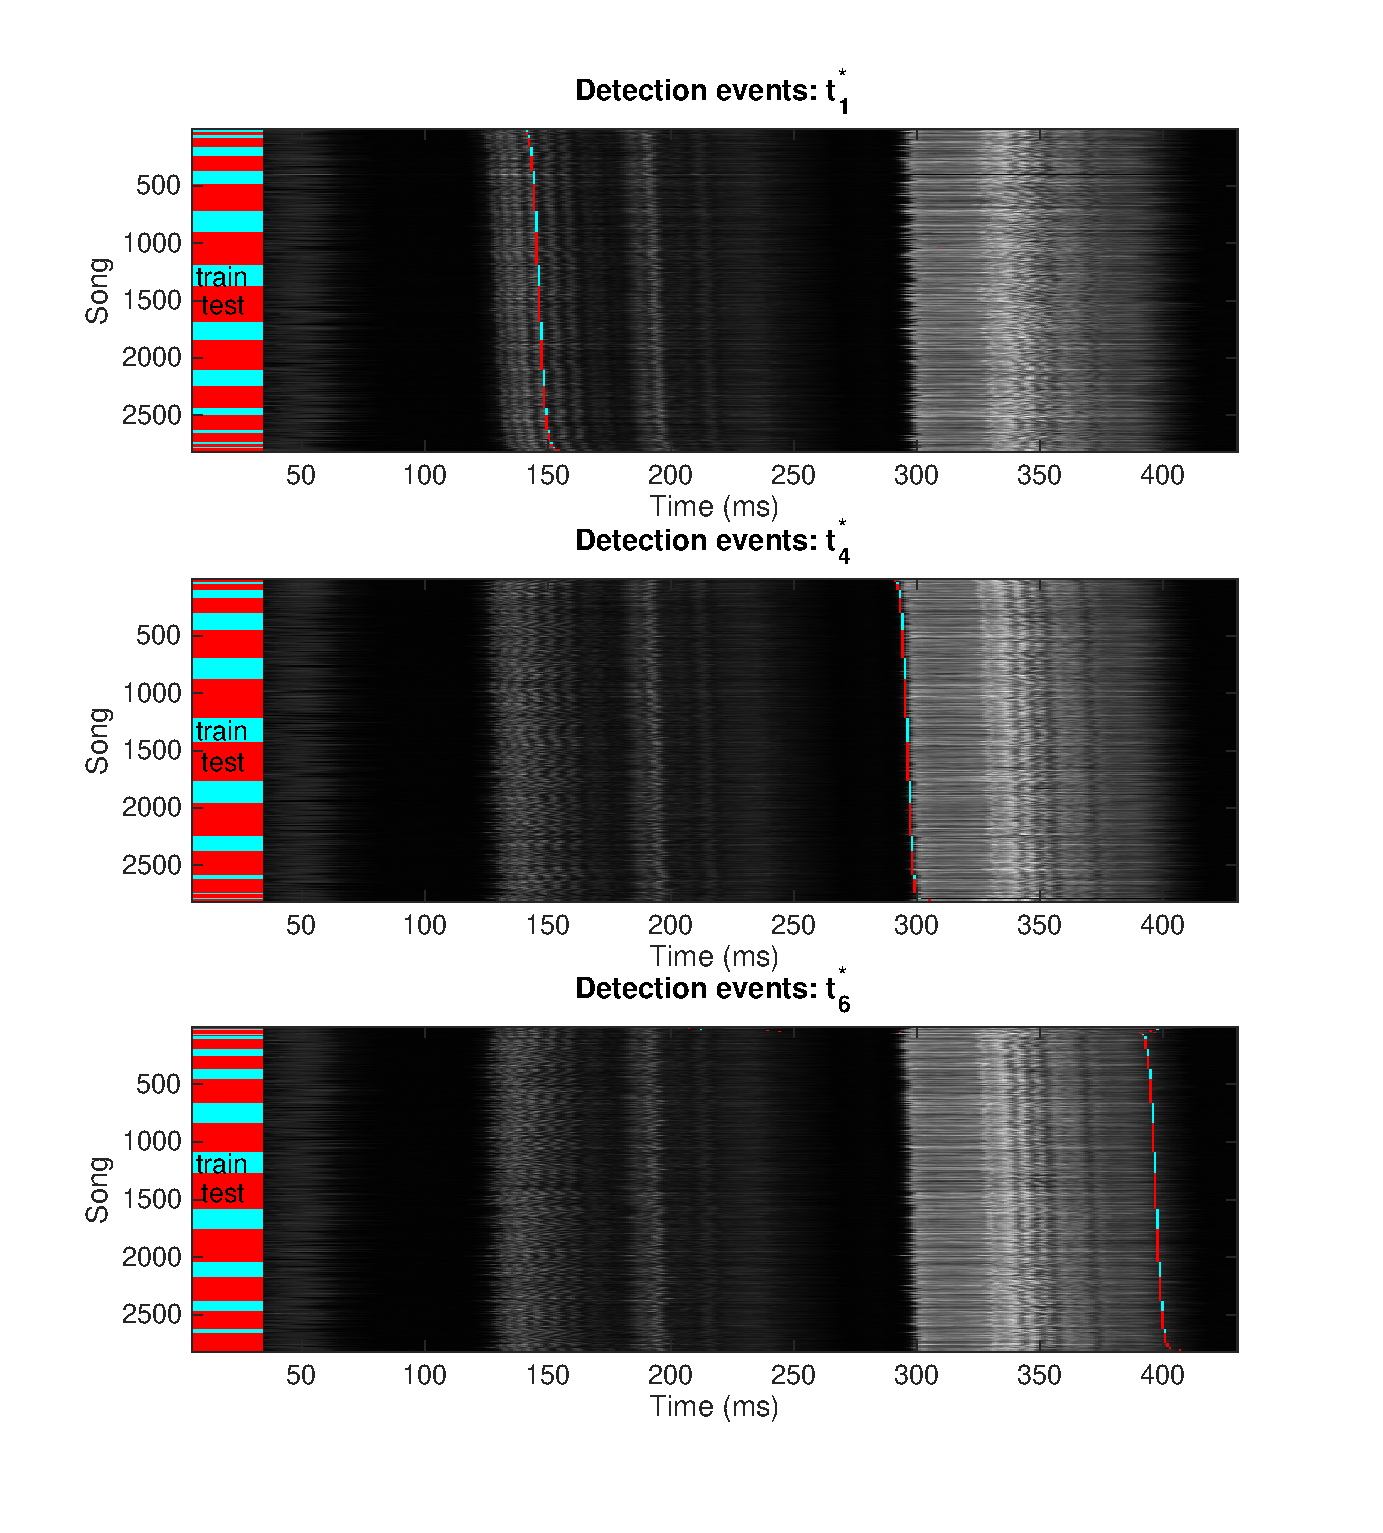
\includegraphics[width=\textwidth]{detection_raster}
  \caption{Each plot shows one network output unit's responses to all
    2818 presentations of the song shown in \fig{fig:song}.  For
    simplicity, we show only the syllables $t^*_2$, $t^*_4$, and $t^*_6$. The
    horizontal axis is time relative to the beginning of the aligned
    song, and the vertical axis is an index for the 2818 single song
    presentations. The grey shading shows the total audio energy of
    song Y at time T. The bar on the left is the same width as the
    detection window, and its colour code shows training songs
    adjacent to cyan regions and unseen test songs adjacent to red
    regions. For visualisation of the distribution, songs have been
    stably sorted by the time of detection events; thus, each of the
    three detection graphs shows the songs in a different order.}
  \label{fig:detection_raster}
\end{figure}

An example of the detector's output for three of these syllables is shown in \fig{fig:detection_raster}.   By sorting according to time of each syllable's detection, the rest of the song is shown in the context of the timing for that moment.  This gives an intuition of the timing variability across different songs (which may be responsible for some of our measured jitter).

\subsection{Accuracy}


\begin{figure}
  \begin{center}
    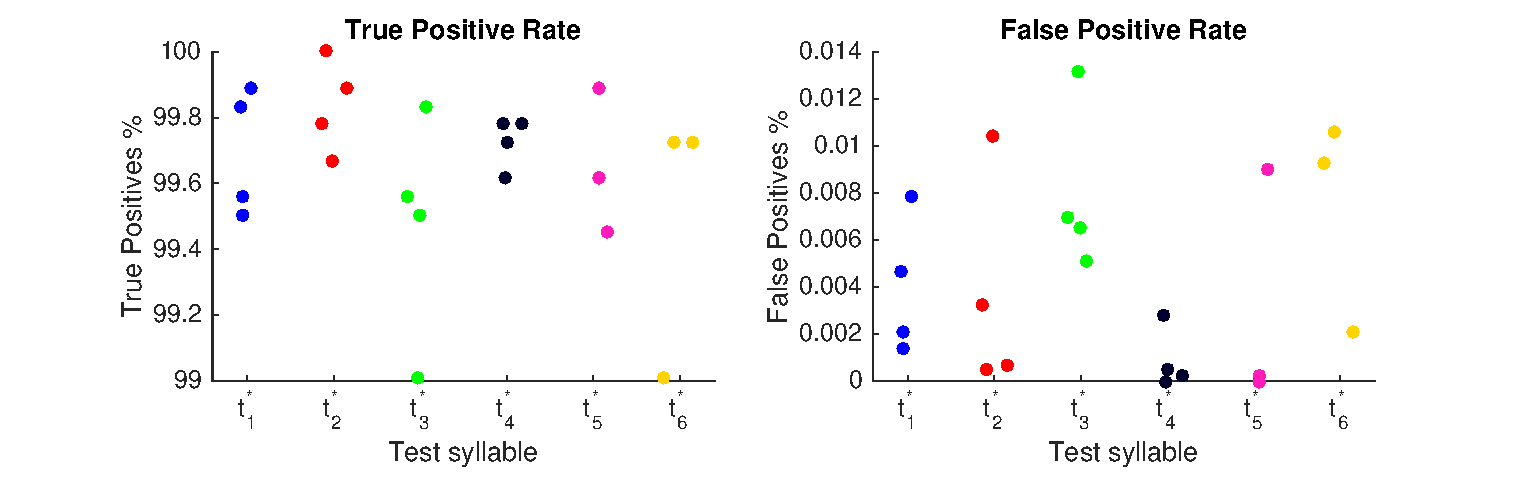
\includegraphics[width=\textwidth]{Accuracies}
  \end{center}
  \caption{Accuracy variability over different training runs for each of the six test syllables.  Each dot shows the test-set accuracy for an independently trained detector.  Because the horizontal positions have been randomised slightly to show same-valued measurements, test syllable is also indicated by colour.}
  \label{fig:accuracies}
\end{figure}


We allowed our training software to allocate our default of 4 hidden units per syllable, and computed a new FFT every 1.5 ms.  Because our timing test files are designed for our stereo playback software, allowing only one channel for the ground-truth pulse, we trained one detector for each syllable for the following results.  In order to eliminate the large number of variables involved in microphone, cage, playback and re-digitising, we evaluated the neural network's accuracy directly on the digitised recording.  When training and runtime data are gathered on the same hardware setup, this is the digital signal that the detector will see---only the non-song data may be different.
%Accuracy \marginpar{Should be! Verify! And/or explain that there is a bug in the LabView implementation, if there in fact is. ALSO need to present a picture of the test syllable or etc\dots} is identical across the three detectors.
\noprint{
  Typical confusion matrices for these syllables are:

  \vspace{8pt}\par\noindent
  \begin{tabular}{r|cc}
    $t^*_1$
    & \multicolumn{2}{c}{True} \\ 
    & pos & neg \\ 
    \hline  Detected pos & 99.96451\% & 0.000298\%\\ 
    neg & 0.0355\% & 99.99970\%\\ 
  \end{tabular}
  \vspace{8pt}\par\noindent
  \begin{tabular}{r|cc}
    $t^*_2$ & \multicolumn{2}{c}{True} \\ 
    & pos & neg \\ 
    \hline  Detected pos & 99.92903\% & 0.000596\%\\ 
    neg & 0.0710\% & 99.99940\%\\ 
  \end{tabular}
  \vspace{8pt}\par\noindent
  \begin{tabular}{r|cc}
    $t^*_3$ & \multicolumn{2}{c}{True} \\ 
    & pos & neg \\ 
    \hline  Detected pos & 99.68062\% & 0.00194\%\\ 
    neg & 0.319\% & 99.99806\%\\ 
  \end{tabular}
  \vspace{8pt}\par\noindent
  \begin{tabular}{r|cc}
    $t^*_4$ & \multicolumn{2}{c}{True} \\ 
    & pos & neg \\ 
    \hline  Detected pos & 99.82257\% & 0.00239\%\\ 
    neg & 0.177\% & 99.99761\%\\ 
  \end{tabular}
  \vspace{8pt}\par\noindent
  \begin{tabular}{r|cc}
    $t^*_5$ & \multicolumn{2}{c}{True} \\ 
    & pos & neg \\ 
    \hline  Detected pos & 99.78708\% & 0\\ 
    neg & 0.213\% & 100\%\\ 
  \end{tabular}
  \vspace{8pt}\par\noindent
  \begin{tabular}{r|cc}
    $t^*_6$ & \multicolumn{2}{c}{True} \\ 
    & pos & neg \\ 
    \hline  Detected pos & 99.71611\% & 0.00552\%\\ 
    neg & 0.284\% & 99.99448\%\\ 
  \end{tabular}
  \vspace{8pt}\par\noindent
}


Accuracies for our six test syllables are shown in \fig{fig:accuracies} (accuracies for the synthetic $\delta$-function songs were always 100\%).  For each test syllable, we trained fifteen\marginpar{FIXME: how many runs in the end?} different networks, which differ from each other in the random initialisation of network weights and on which random subset of our songs was used for training.  Each network's accuracy is shown as a single point in each chart in \fig{fig:accuracies}.  Some syllables are easier to identify reliably than others, allowing detection point choice to impact the detector's accuracy.  For difficult syllables, the training process occasionally yields a network that performs unusually poorly, but it is easy to spot these networks by their performance on the test audio file, and re-train when necessary.


\subsection{Timing}

We evaluate variability in timing performance across three variables: FFT frame interval; syllable choice; and detector implementation.

\subsubsection{FFT Frame Interval}

\begin{figure}
  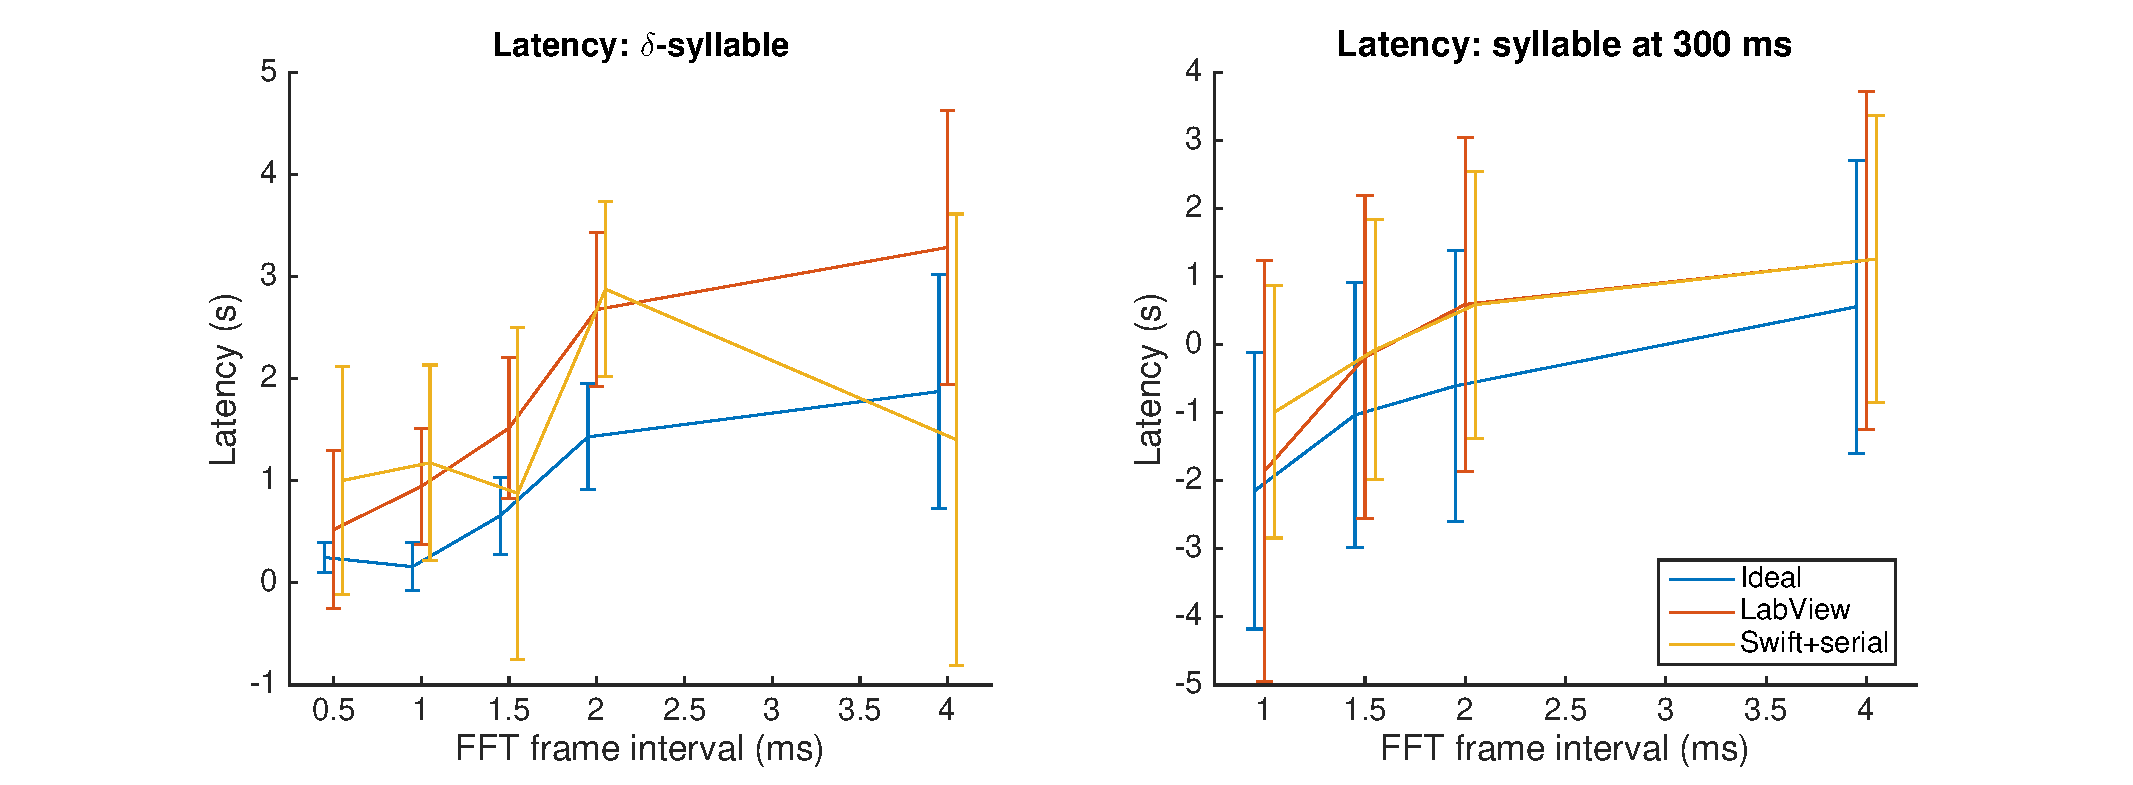
\includegraphics[width=\textwidth]{TimingVsFrame}
  \caption{Timing varies as the FFT frame interval changes.  Here we show results for the ideal detector and the LabView and Swift+serial implementations, for the constructed $\delta$-syllable and for trigger $t^*_4$ of the bird song.  The lines show latency, with errorbars reprenting jitter.  Points have been shifted slightly for clarity; original positions are [0.5 1 1.5 2 4] ms.}
  \label{fig:TimingVsFrame}
\end{figure}

Detector latency and jitter depend on the FFT frame rate.  Our 1.5-ms--frame default is a compromise: shorter frames increase the precision of timing, but also increase computational requirements both during training and at runtime.  \fig{fig:TimingVsFrame} shows how these numbers vary over a useful range of frame rates on our ideal detector, the Swift detector with serial output, and for the LabView detector, for both the $\delta$-syllable and for the bird song at $t^*_4$.

\subsubsection{Syllable choice}

\begin{figure}
  \begin{center}
    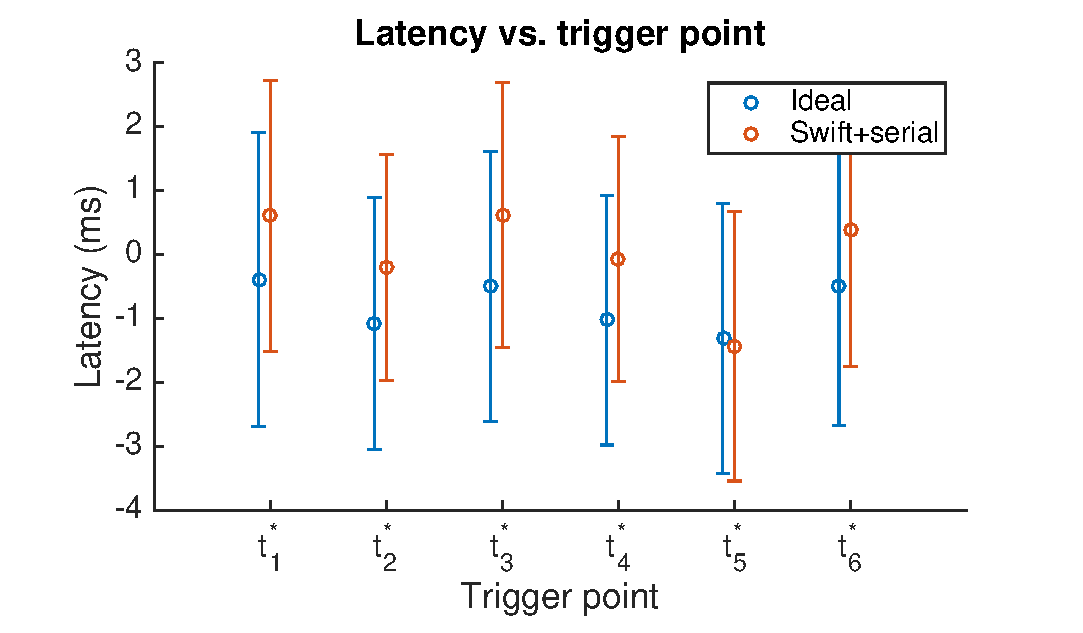
\includegraphics[width=8cm]{TimingVsSyllable}
  \end{center}
  \caption{Timing data for our 6 test syllables, for the ideal and the Swift+serial detectors, with an FFT frame rate of 1.5 ms.  Point centres show latency; error bars show jitter.}
  \label{fig:TimingVsSyllable}
\end{figure}

Syllable choice impacts detector performance, but despite the variety of syllables chosen here, performance was fairly stable across syllables.  \fig{fig:TimingVsSyllable} shows measured timing data for the Swift+serial detector compared to the ideal, with $t_{\textrm{fft}}=1.5$ ms.  Given the variety of the test syllables, the variability is surprisingly low, and is summarised here with 95\% confidence intervals (with n=6):
\vspace{8pt}\par\noindent
\begin{tabular}{r|cc}
  Detector & Latency & Jitter \\ 
  \hline   Ideal & $-0.8\pm 0.3$ ms & $2.1\pm 0.1$ ms \\
  Swift+serial & $0.0\pm 0.6$ ms & $2.0\pm 0.1$ ms
\end{tabular}
\vspace{8pt}\par\noindent
The negative latency is due to the way in which the network responds to the song through time: as the recognition region looks increasingly similar to the trained match, the network's evaluation of similarity rises, and will generally cross the triggering threshold before it reaches its maximum value.  A heuristic as simple as triggering at an apparent turning point after crossing the threshold might improve timing consistency, but we did not test this.

\subsubsection{Detector Implementations}

\begin{figure}
  \begin{center}
    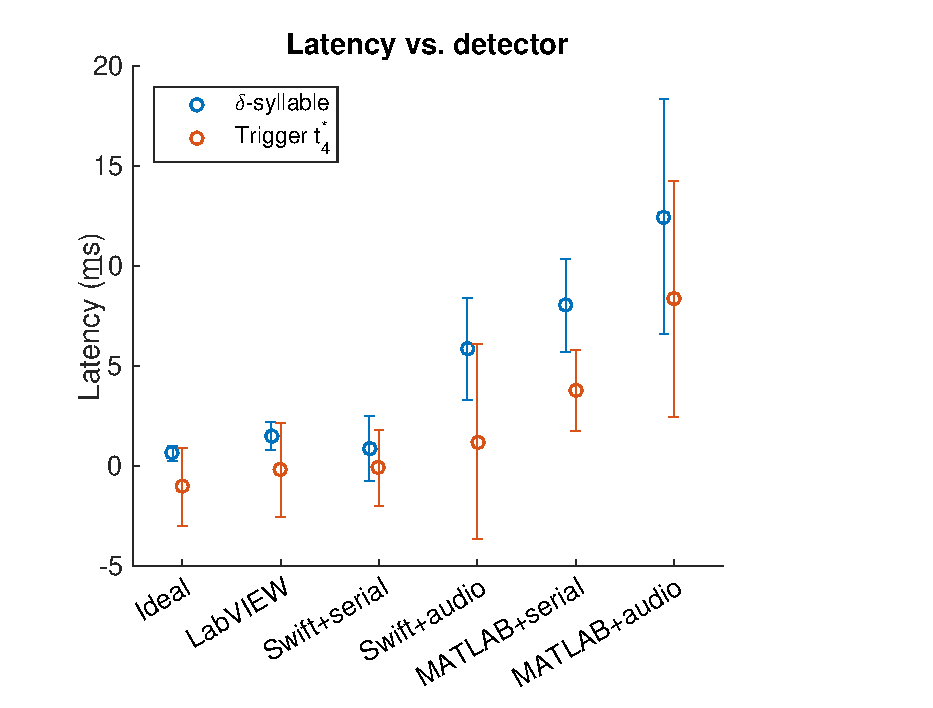
\includegraphics[width=8cm]{TimingVsDetector}
  \end{center}
  \caption{The different detectors for the constructed $\delta$-syllable and for the bird song at $t^*_4$.  Point centres show latency; error bars show jitter.}
  \label{fig:TimingVsDetector}
\end{figure}

\begin{figure}
  \begin{center}
    \includegraphics[width=8cm]{timing}
  \end{center}
  \caption{Raw timing curves for all detectors measured during detection of $t^*_4$ using 1.5-ms frames.  A maximum-likelihood fit of a Gaussian cumumative distribution function was computed for each curve, from which were extracted the mean---latency---and standard deviation---jitter.}
  \label{fig:timing}
\end{figure}

We compared latency and jitter across our different detector implementations for the $\delta$-syllable and $t^*_4$, again with $t_\mathrm{fft}=1.5$ ms.  Results are as follows:
\vspace{8pt}
\begin{tabular}{l|c|c|c| c}
  & \multicolumn{2}{c}{$\delta$-syllable} & \multicolumn{2}{c}{Bird: $t^*_4$} \\
  Detector & Latency (ms) & Jitter (ms) & Latency (ms) & Jitter (ms) \\
  \hline
  Ideal & 0.66 & 0.38 & -1.0 & 2.0 \\
  LabView & 1.5 & 0.69 & -0.18 & 2.4 \\
  Swift+serial & 0.88 & 1.6 & -0.075 & 2.0 \\
  Swift+audio & 5.89 & 2.6 & 1.24 & 4.9 \\
  Matlab+serial & 8.1 & 2.3 & 3.8 & 2.0 \\
  Matlab+audio & 12.5 & 5.9 & 8.4 & 5.9
\end{tabular}
\vspace{8pt}\par\noindent
These data are also plotted in \fig{fig:TimingVsDetector}, and \fig{fig:timing} gives a more detailed view of what the timing curves look like for the five implementations of our detector on $t^*_4$.


\section{Discussion}
\label{sec:conclusion}

This syllable detector is appropriate for zebra finch song, and although our tests were carried out on songs from that species, it is also likely to work well for Bengalese finches.  It offers the following benefits:
\begin{itemize}
\item The detector is accurate. False negative and
  false positive rates can be well under 0.5\% and 0.01\% respectively, and trading these two numbers off against each other is through a single relative-cost parameter.
\item Latency is generally under a millisecond, with jitter around 2 ms.
\item Works on a wide range of target syllables using the default values described here, generally eliminating the need for hand-tuning.
\item Runs fast enough for syllable-modification experiments on inexpensive consumer-grade hardware, although we recommend that the training phase be run on a fast desktop system with 32 GB of RAM.
\item A single detector can generate different target pulses for multiple syllables at almost no additional computational cost during runtime, although training time will increase.
\end{itemize}

Although there are differences, the Swift+serial detector and the LabView implementation are roughly comparable in performance.  We prefer the Swift implementation due to its lower hardware and software requirements and the difficulty of debugging LabView programmes.  With serial output, Matlab's performance is good, although its buffer handling is sensitive to system load.

The song presented here was recorded with a fixed microphone mounted inside the cage.  We found that higher accuracy is achieved when a microphone is instead mounted on the bird's head, which maintains volume and reduces changes in timbre as the bird moves.

A common experimental paradigm requires detecting the frequency of syllables.  Many pitch detection techniques rely on the spectrum, which incurs no additional computational cost here since it is already available.  For example, \cite{Canopoli2014} achieved good results with the Harmonic Product Spectrum algorithm \cite{Noll1970pitchdetection}.

In order to monitor syllable duration, the beginning and end of a syllable may be detected by looking at the ratio of total energy in the singing frequency band to the total energy, over some small time window.  Any syllable thus identified that also contains a trigger event may be monitored for duration.  Alternatively, the network can be trained to recognise both the beginning and the end of the syllable of interest.

In feedback experiments such as frequency- or duration-shifting, vocal output changes over the course of the experiment.  The neural network excels at identifying syllables close to its training set, so as vocal output changes the detector may not recognise a match.  If the detector must be robust to this shift, it may be retrained as often as necessary as the bird learns, or data consisting of synthetically pitch-shifted or duration-shifted target syllables over the recognition region may be added to the training set.  We will test these approaches in future work.

\section{Acknowledgments}
We would like to thank William A.~Liberti for his improvements to the draft.
This work was funded by NIH grants 5R01NS089679-02 and 5U01NS090454-02.

\appendix

\section{Resources}
\label{sec:resources}
\marginpar{PLOS doesn't really say where such things should go.}
\marginpar{Cleanup: mostly done.  But it would be nice to move all this to the lab's github group.}
\begin{description}
  \item[Song alignment:] Last we checked, Jeff Markowitz's song
    alignment software could be found at \\
    {\tt https://github.com/jmarkow}.

    \item[Training the neural network:] Our implementation of the syllable
      detector training code is available under the GNU GPL at:
      \\ {\tt https://github.com/bwpearre/}

    \item[Runtime:] The Matlab, Swift, and Labview implementations for executing the trained
      network:\\
      {\tt https://github.com/nathanntg/syllable-detector}
\end{description}

\bibliography{birds}

\end{document}

